\documentclass[journal,12pt,twocolumn]{IEEEtran}
%\usepackage{setspace}
\usepackage{gensymb}
%\doublespacing
%\singlespacing

\usepackage{tikz}
\usetikzlibrary{decorations.markings}
\newif\iflabrev
%\usepackage{graphicx}
%\usepackage{amssymb}
%\usepackage{relsize}
\usepackage[cmex10]{amsmath}
%\usepackage{amsthm}
%\interdisplaylinepenalty=2500
%\savesymbol{iint}
%\usepackage{txfonts}
%\restoresymbol{TXF}{iint}
%\usepackage{wasysym}
\usepackage{amsthm}
%\usepackage{iithtlc}
\usepackage{mathrsfs}
\usepackage{txfonts}
\usepackage{stfloats}
\usepackage{bm}
\usepackage{cite}
\usepackage{cases}
\usepackage{subfig}
%\usepackage{xtab}
\usepackage{longtable}
\usepackage{multirow}
%\usepackage{algorithm}
%\usepackage{algpseudocode}
\usepackage{enumitem}
\usepackage{mathtools}
\usepackage{tikz}
\usepackage{circuitikz}
\usepackage{verbatim}
%\usepackage{tfrupee}
%\usepackage[breaklinks=true]{hyperref}
%\usepackage{stmaryrd}
%\usepackage{tkz-euclide} % loads  TikZ and tkz-base
%\usetkzobj{all}
%\usepackage{listings}
    \usepackage{color}                                            %%
    \usepackage{array}                                            %%
    \usepackage{longtable}                                        %%
    \usepackage{calc}                                             %%
    \usepackage{multirow}                                         %%
    \usepackage{hhline}                                           %%
    \usepackage{ifthen}                                           %%
  %optionally (for landscape tables embedded in another document): %%
    \usepackage{lscape}     
\usepackage{multicol}
\usepackage{chngcntr}
%\usepackage{enumerate}

%\usepackage{wasysym}
%\newcounter{MYtempeqncnt}
\DeclareMathOperator*{\Res}{Res}
%\renewcommand{\baselinestretch}{2}
\renewcommand\thesection{\arabic{section}}
\renewcommand\thesubsection{\thesection.\arabic{subsection}}
\renewcommand\thesubsubsection{\thesubsection.\arabic{subsubsection}}

\renewcommand\thesectiondis{\arabic{section}}
\renewcommand\thesubsectiondis{\thesectiondis.\arabic{subsection}}
\renewcommand\thesubsubsectiondis{\thesubsectiondis.\arabic{subsubsection}}

% correct bad hyphenation here
\hyphenation{op-tical net-works semi-conduc-tor}
\def\inputGnumericTable{}                                 %%

%\lstset{
%language=C,
%frame=single, 
%breaklines=true,
%columns=fullflexible
%}
%\lstset{
%language=tex,
%frame=single, 
%breaklines=true
%}

\begin{document}
%


\newtheorem{theorem}{Theorem}[section]
\newtheorem{problem}{Problem}
\newtheorem{proposition}{Proposition}[section]
\newtheorem{lemma}{Lemma}[section]
\newtheorem{corollary}[theorem]{Corollary}
\newtheorem{example}{Example}[section]
\newtheorem{definition}[problem]{Definition}
%\newtheorem{thm}{Theorem}[section] 
%\newtheorem{defn}[thm]{Definition}
%\newtheorem{algorithm}{Algorithm}[section]
%\newtheorem{cor}{Corollary}
\newcommand{\BEQA}{\begin{eqnarray}}
\newcommand{\EEQA}{\end{eqnarray}}
\newcommand{\define}{\stackrel{\triangle}{=}}
\bibliographystyle{IEEEtran}
%\bibliographystyle{ieeetr}
\providecommand{\mbf}{\mathbf}
\providecommand{\pr}[1]{\ensuremath{\Pr\left(#1\right)}}
\providecommand{\qfunc}[1]{\ensuremath{Q\left(#1\right)}}
\providecommand{\sbrak}[1]{\ensuremath{{}\left[#1\right]}}
%\providecommand{\lsbrak}[1]{\ensuremath{{}\left[#1\right.}}
\providecommand{\rsbrak}[1]{\ensuremath{{}\left.#1\right]}}
%\providecommand{\brak}[1]{\ensuremath{\left(#1\right)}}
\providecommand{\lbrak}[1]{\ensuremath{\left(#1\right.}}
\providecommand{\rbrak}[1]{\ensuremath{\left.#1\right)}}
\providecommand{\cbrak}[1]{\ensuremath{\left\{#1\right\}}}
\providecommand{\lcbrak}[1]{\ensuremath{\left\{#1\right.}}
\providecommand{\rcbrak}[1]{\ensuremath{\left.#1\right\}}}
\theoremstyle{remark}
\newtheorem{rem}{Remark}
\newcommand{\sgn}{\mathop{\mathrm{sgn}}}
\providecommand{\abs}[1]{\left\vert#1\right\vert}
\providecommand{\res}[1]{\Res\displaylimits_{#1}} 
\providecommand{\norm}[1]{\left\lVert#1\right\rVert}
%\providecommand{\norm}[1]{\lVert#1\rVert}
\providecommand{\mtx}[1]{\mathbf{#1}}
\providecommand{\mean}[1]{E\left[ #1 \right]}
\providecommand{\fourier}{\overset{\mathcal{F}}{ \rightleftharpoons}}
%\providecommand{\hilbert}{\overset{\mathcal{H}}{ \rightleftharpoons}}
\providecommand{\system}{\overset{\mathcal{H}}{ \longleftrightarrow}}
	%\newcommand{\solution}[2]{\textbf{Solution:}{#1}}
\newcommand{\solution}{\noindent \textbf{Solution: }}
\newcommand{\cosec}{\,\text{cosec}\,}
\providecommand{\dec}[2]{\ensuremath{\overset{#1}{\underset{#2}{\gtrless}}}}
\newcommand{\myvec}[1]{\ensuremath{\begin{pmatrix}#1\end{pmatrix}}}
\newcommand{\mydet}[1]{\ensuremath{\begin{vmatrix}#1\end{vmatrix}}}
%\numberwithin{equation}{section}
\numberwithin{equation}{subsection}
%\numberwithin{problem}{section}
%\numberwithin{definition}{section}
\makeatletter
\@addtoreset{figure}{problem}
\makeatother

\let\StandardTheFigure\thefigure
\let\vec\mathbf
%\renewcommand{\thefigure}{\theproblem.\arabic{figure}}
\renewcommand{\thefigure}{\theproblem}
%\setlist[enumerate,1]{before=\renewcommand\theequation{\theenumi.\arabic{equation}}
%\counterwithin{equation}{enumi}


%\renewcommand{\theequation}{\arabic{subsection}.\arabic{equation}}

\def\putbox#1#2#3{\makebox[0in][l]{\makebox[#1][l]{}\raisebox{\baselineskip}[0in][0in]{\raisebox{#2}[0in][0in]{#3}}}}
     \def\rightbox#1{\makebox[0in][r]{#1}}
     \def\centbox#1{\makebox[0in]{#1}}
     \def\topbox#1{\raisebox{-\baselineskip}[0in][0in]{#1}}
     \def\midbox#1{\raisebox{-0.5\baselineskip}[0in][0in]{#1}}

\vspace{3cm}

\title{
	\logo{
Control Systems
	}
}
\author{ G V V Sharma$^{*}$% <-this % stops a space
	\thanks{*The author is with the Department
		of Electrical Engineering, Indian Institute of Technology, Hyderabad
		502285 India e-mail:  gadepall@iith.ac.in. All content in this manual is released under GNU GPL.  Free and open source.}
	
}	
%\title{
%	\logo{Matrix Analysis through Octave}{\begin{center}\includegraphics[scale=.24]{tlc}\end{center}}{}{HAMDSP}
%}


% paper title
% can use linebreaks \\ within to get better formatting as desired
%\title{Matrix Analysis through Octave}
%
%
% author names and IEEE memberships
% note positions of commas and nonbreaking spaces ( ~ ) LaTeX will not break
% a structure at a ~ so this keeps an author's name from being broken across
% two lines.
% use \thanks{} to gain access to the first footnote area
% a separate \thanks must be used for each paragraph as LaTeX2e's \thanks
% was not built to handle multiple paragraphs
%

%\author{<-this % stops a space
%\thanks{}}
%}
% note the % following the last \IEEEmembership and also \thanks - 
% these prevent an unwanted space from occurring between the last author name
% and the end of the author line. i.e., if you had this:
% 
% \author{....lastname \thanks{...} \thanks{...} }
%                     ^------------^------------^----Do not want these spaces!
%
% a space would be appended to the last name and could cause every name on that
% line to be shifted left slightly. This is one of those "LaTeX things". For
% instance, "\textbf{A} \textbf{B}" will typeset as "A B" not "AB". To get
% "AB" then you have to do: "\textbf{A}\textbf{B}"
% \thanks is no different in this regard, so shield the last } of each \thanks
% that ends a line with a % and do not let a space in before the next \thanks.
% Spaces after \IEEEmembership other than the last one are OK (and needed) as
% you are supposed to have spaces between the names. For what it is worth,
% this is a minor point as most people would not even notice if the said evil
% space somehow managed to creep in.



% The paper headers
%\markboth{Journal of \LaTeX\ Class Files,~Vol.~6, No.~1, January~2007}%
%{Shell \MakeLowercase{\textit{et al.}}: Bare Demo of IEEEtran.cls for Journals}
% The only time the second header will appear is for the odd numbered pages
% after the title page when using the twoside option.
% 
% *** Note that you probably will NOT want to include the author's ***
% *** name in the headers of peer review papers.                   ***
% You can use \ifCLASSOPTIONpeerreview for conditional compilation here if
% you desire.




% If you want to put a publisher's ID mark on the page you can do it like
% this:
%\IEEEpubid{0000--0000/00\$00.00~\copyright~2007 IEEE}
% Remember, if you use this you must call \IEEEpubidadjcol in the second
% column for its text to clear the IEEEpubid mark.



% make the title area
%\maketitle

\newpage

\tableofcontents

\bigskip

\renewcommand{\thefigure}{\theenumi}
\renewcommand{\thetable}{\theenumi}
%\renewcommand{\theequation}{\theenumi}

%\begin{abstract}
%%\boldmath
%In this letter, an algorithm for evaluating the exact analytical bit error rate  (BER)  for the piecewise linear (PL) combiner for  multiple relays is presented. Previous results were available only for upto three relays. The algorithm is unique in the sense that  the actual mathematical expressions, that are prohibitively large, need not be explicitly obtained. The diversity gain due to multiple relays is shown through plots of the analytical BER, well supported by simulations. 
%
%\end{abstract}
% IEEEtran.cls defaults to using nonbold math in the Abstract.
% This preserves the distinction between vectors and scalars. However,
% if the journal you are submitting to favors bold math in the abstract,
% then you can use LaTeX's standard command \boldmath at the very start
% of the abstract to achieve this. Many IEEE journals frown on math
% in the abstract anyway.

% Note that keywords are not normally used for peerreview papers.
%\begin{IEEEkeywords}
%Cooperative diversity, decode and forward, piecewise linear
%\end{IEEEkeywords}



% For peer review papers, you can put extra information on the cover
% page as needed:
% \ifCLASSOPTIONpeerreview
% \begin{center} \bfseries EDICS Category: 3-BBND \end{center}
% \fi
%
% For peerreview papers, this IEEEtran command inserts a page break and
% creates the second title. It will be ignored for other modes.
%\IEEEpeerreviewmaketitle

\begin{abstract}
This manual is an introduction to control systems based on GATE problems.Links to sample Python codes are available in the text.  
\end{abstract}
Download python codes using 
%\begin{lstlisting}
%svn co https://github.com/gadepall/school/trunk/control/codes
%\end{lstlisting}

%\section{Bode Plot}
%\begin{enumerate}[label=\thesection.\arabic*.,ref=\thesection.\theenumi]
%\numberwithin{equation}{enumi}
%\input{./chapters/ee18btech11001.tex}
%\end{enumerate}
\section{Stability}
\subsection{Second order System}
%\input{./chapters/ee18btech11002.tex}
\begin{enumerate}[label=\thesection.\arabic*.,ref=\thesection.\theenumi]
\numberwithin{equation}{enumi}

\item The Block diagram of a system is illustrated in the figure shown, where $X(s)$ is the input and $Y(s)$ is the output. Draw the equivalent signal flow graph.
\renewcommand{\thefigure}{\theenumi.\arabic{figure}}

\begin{figure}[!ht]
    \tikzstyle{block} = [draw, fill=white, rectangle, 
minimum height=2em, minimum width=3em]
\tikzstyle{sum} = [draw, fill=white, circle, radius=1mm, node distance=1.5cm]
\tikzstyle{input} = [coordinate]
\tikzstyle{output} = [coordinate]
\tikzstyle{pinstyle} = [pin edge={to-,thin,black}]

\begin{tikzpicture}[auto, node distance=2cm,>=latex']
\node [input, name=input] {};
\node [sum, right of=input] (sum1) {$\sum$};
\node [input, right of=sum1] (B1) {};
\node [input, right of=B1] (B2) {};
\node [block, below of=B2] (B3) {$\frac{1}{s}$};
\node [block, above of=B2] (B4) {$s$};
\node [sum, right of=B2] (B5) {$\sum$};
\node [input, right of=B5] (B6) {};
\node [input, above of=B6] (A1) {};
\node [input, above of=A1] (A2) {};
\node [block, right of=B6] (B7) {$\frac{1}{s}$};
\node [input, right of=B7] (B8) {};
\node [input, below of=B8] (A3) {};
\node [input, below of=A3] (A4) {};
\node [output, right of=B8] (output) {};

\draw [->] (input)--node[pos=0.00]{$X(s)$} node[pos=0.99]{$+$}(sum1);
\draw[-] (sum1)--(B1);
\draw[->](B1) |- node[pos=0.99] {} (B4);
\draw[->](B1) |- node[pos=0.99] {} (B3);
\draw [->](B4) -| node[pos=0.99] {$+$} (B5);
\draw [->](B3) -| node[pos=0.99] {$+$} (B5);
\draw [->](B5)--(B7);
\draw [-](B7)--(B8);
\draw [->](B8)--node[pos=0.99] {$Y(s)$} (output);
\draw [-](B6) -- (A2);
\draw [->](A2) -| node[pos=0.99] {$-$} (sum1);
\draw [-](B8)--(A4);
\draw [->](A4) -| node[pos=0.99] {$-$} (sum1);

\end{tikzpicture}
\caption{signal flow graph}
\label{fig:sec_order}
\end{figure}
\solution
Signal flow graph of given above block diagram is
\begin{figure}[!ht]
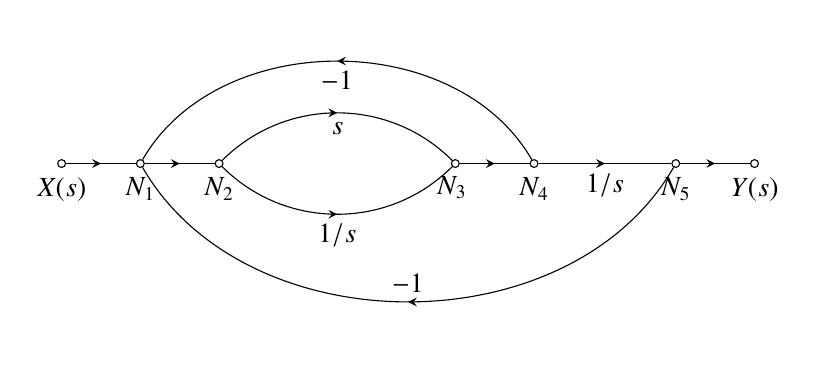
\begin{tikzpicture}
[
label revd/.is if=labrev,
amark/.style={
            decoration={             
                        markings,   
                        mark=at position {0.5} with { 
                                    \arrow{stealth},
                                    \iflabrev \node[above] {#1};\else \node[below] {#1};\fi
                        }
            },
            postaction={decorate}
},
terminal/.style 2 args={draw,circle,inner sep=1pt,label={#1:#2}},
]

%Place the nodes
\node[terminal={below}{$X(s)$}] (a) at (0,0) {};
\node[terminal={below}{$N_1$}] (b) at (1cm,0) {};
\node[terminal={below}{$N_2$}] (c) at (2cm,0) {};
\node[terminal={[xshift=-4mm]below right}{$N_3$}] (d) at (5cm,0) {};
\node[terminal={below}{$N_4$}] (e) at (6cm,0) {};
\node[terminal={below}{$N_5$}] (f) at (7.8cm,0) {};
\node[terminal={below}{$Y(s)$}] (g) at (8.8cm,0) {};
%Draw the connections
\draw[amark=$ $] (a) to (b);
\draw[amark=$ $] (b) to (c);
\draw[amark=$s$] (c) to[bend left=45] (d);
\draw[amark=$1/s$] (e) to (f);
\draw[amark=$ $] (f) to (g);
\draw[amark=$ $] (d) to (e);
\draw[amark=$1/s$] (c) to[bend left=-45] (d);
\draw[amark=$-1$] (e) to[bend left=-60] (b);
\draw[amark=$-1$,label revd] (f) to[bend left=60] (b);
%\draw[amark=$-K/M$,label revd] (e) to[bend right=50] (c);
\end{tikzpicture}
\caption{signal flow graph}
\label{fig:sec_order}
\end{figure}
%
\renewcommand{\thefigure}{\theenumi}
\item Draw all the forward paths and compute the respective gains.
\renewcommand{\thefigure}{\theenumi.\arabic{figure}}
\solution
Here, 
\begin{align}
P_1=\frac{s}{s}=1
\end{align}

\begin{figure}[!ht]
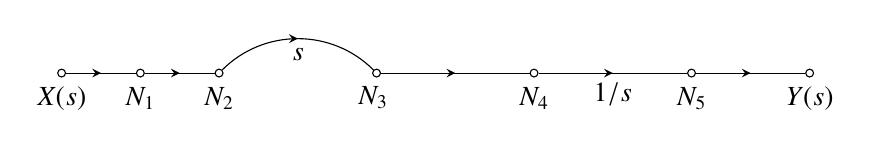
\begin{tikzpicture}
[
label revd/.is if=labrev,
amark/.style={
            decoration={             
                        markings,   
                        mark=at position {0.5} with { 
                                    \arrow{stealth},
                                    \iflabrev \node[above] {#1};\else \node[below] {#1};\fi
                        }
            },
            postaction={decorate}
},
terminal/.style 2 args={draw,circle,inner sep=1pt,label={#1:#2}},
]

%Place the nodes
\node[terminal={below}{$X(s)$}] (a) at (0,0) {};
\node[terminal={below }{$N_1$}] (b) at (1cm,0) {};
\node[terminal={below }{$N_2$}] (c) at (2cm,0) {};
\node[terminal={[xshift=-4mm]below right}{$N_3$}] (d) at (4cm,0) {};
\node[terminal={below }{$N_4$}] (e) at (6cm,0) {};
\node[terminal={below }{$N_5$}] (f) at (8cm,0) {};
\node[terminal={below }{$Y(s)$}] (g) at (9.5cm,0) {};
%Draw the connections
\draw[amark=$ $] (a) to (b);
\draw[amark=$ $] (b) to (c);
\draw[amark=$s$] (c) to[bend left=45] (d);
\draw[amark=$1/s$] (e) to (f);
\draw[amark=$ $] (f) to (g);
\draw[amark=$ $] (d) to (e);
%\draw[amark=$1/s$] (c) to[bend left=-45] (d);
%\draw[amark=$-1$] (e) to[bend left=-45] (b);
%\draw[amark=$-1$,label revd] (f) to[bend left=50] (b);
%\draw[amark=$-K/M$,label revd] (e) to[bend right=50] (c);
\end{tikzpicture}
\caption{$P_1$}
\label{fig:sec_order}
\end{figure}

 
\begin{align}
P_2=(1/s)(1/s)=1/s^2
\end{align}

\begin{figure}[!ht]
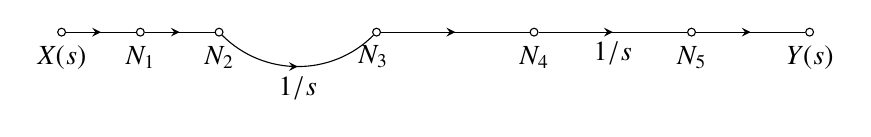
\begin{tikzpicture}
[
label revd/.is if=labrev,
amark/.style={
            decoration={             
                        markings,   
                        mark=at position {0.5} with { 
                                    \arrow{stealth},
                                    \iflabrev \node[above] {#1};\else \node[below] {#1};\fi
                        }
            },
            postaction={decorate}
},
terminal/.style 2 args={draw,circle,inner sep=1pt,label={#1:#2}},
]

%Place the nodes
\node[terminal={below}{$X(s)$}] (a) at (0,0) {};
\node[terminal={below }{$N_1$}] (b) at (1cm,0) {};
\node[terminal={below }{$N_2$}] (c) at (2cm,0) {};
\node[terminal={[xshift=-4mm]below right}{$N_3$}] (d) at (4cm,0) {};
\node[terminal={below }{$N_4$}] (e) at (6cm,0) {};
\node[terminal={below }{$N_5$}] (f) at (8cm,0) {};
\node[terminal={below }{$Y(s)$}] (g) at (9.5cm,0) {};
%Draw the connections
\draw[amark=$ $] (a) to (b);
\draw[amark=$ $] (b) to (c);
%\draw[amark=$s$] (c) to[bend left=45] (d);
\draw[amark=$1/s$] (e) to (f);
\draw[amark=$ $] (f) to (g);
\draw[amark=$ $] (d) to (e);
\draw[amark=$1/s$] (c) to[bend left=-45] (d);
%\draw[amark=$-1$] (e) to[bend left=-45] (b);
%\draw[amark=$-1$,label revd] (f) to[bend left=50] (b);
%\draw[amark=$-K/M$,label revd] (e) to[bend right=50] (c);
\end{tikzpicture}
\caption{$P_2$}
\label{fig:sec_order}
\end{figure}
\renewcommand{\thefigure}{\theenumi}

\item Draw the loops and calculate the respective gains.\renewcommand{\thefigure}{\theenumi.\arabic{figure}}
\\
\solution 
\begin{align}
L_1=(-1)(s)=-s
\end{align}

\begin{figure}[!ht]
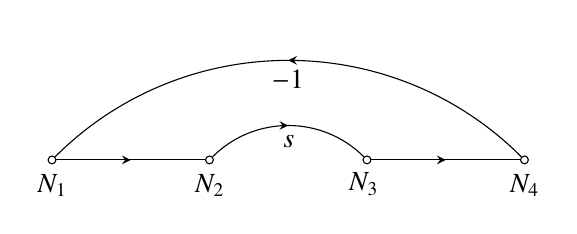
\begin{tikzpicture}
[
label revd/.is if=labrev,
amark/.style={
            decoration={             
                        markings,   
                        mark=at position {0.5} with { 
                                    \arrow{stealth},
                                    \iflabrev \node[above] {#1};\else \node[below] {#1};\fi
                        }
            },
            postaction={decorate}
},
terminal/.style 2 args={draw,circle,inner sep=1pt,label={#1:#2}},
]

%Place the nodes
%\node[terminal={below}{$X(s)$}] (a) at (0,0) {};
\node[terminal={below }{$N_1$}] (b) at (2cm,0) {};
\node[terminal={below }{$N_2$}] (c) at (4cm,0) {};
\node[terminal={[xshift=-4mm]below right}{$N_3$}] (d) at (6cm,0) {};
\node[terminal={below }{$N_4$}] (e) at (8cm,0) {};
%\node[terminal={below left}{$N_5$}] (f) at (11cm,0) {};
%\node[terminal={below left}{$Y(s)$}] (g) at (13cm,0) {};
%Draw the connections
%\draw[amark=$ $] (a) to (b);
\draw[amark=$ $] (b) to (c);
\draw[amark=$s$] (c) to[bend left=45] (d);
%\draw[amark=$1/s$] (e) to (f);
%\draw[amark=$ $] (f) to (g);
\draw[amark=$ $] (d) to (e);
%\draw[amark=$1/s$] (c) to[bend left=-45] (d);
\draw[amark=$-1$] (e) to[bend left=-45] (b);
%\draw[amark=$-1$,label revd] (f) to[bend left=50] (b);
%\draw[amark=$-K/M$,label revd] (e) to[bend right=50] (c);
\end{tikzpicture}
\caption{$L_1$}
\label{fig:sec_order}
\end{figure}


\begin{align}
L_2=\frac{s}{-s}=-1
\end{align}

\begin{figure}[!ht]
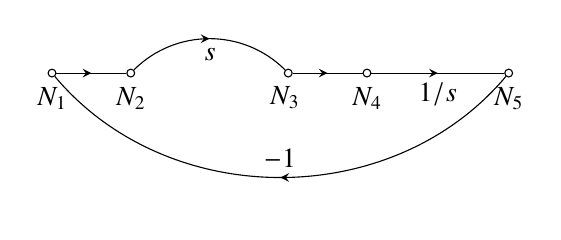
\begin{tikzpicture}
[
label revd/.is if=labrev,
amark/.style={
            decoration={             
                        markings,   
                        mark=at position {0.5} with { 
                                    \arrow{stealth},
                                    \iflabrev \node[above] {#1};\else \node[below] {#1};\fi
                        }
            },
            postaction={decorate}
},
terminal/.style 2 args={draw,circle,inner sep=1pt,label={#1:#2}},
]

%Place the nodes
%\node[terminal={below}{$X(s)$}] (a) at (0,0) {};
\node[terminal={below}{$N_1$}] (b) at (0,0) {};
\node[terminal={below}{$N_2$}] (c) at (1cm,0) {};
\node[terminal={[xshift=-4mm]below right}{$N_3$}] (d) at (3cm,0) {};
\node[terminal={below}{$N_4$}] (e) at (4cm,0) {};
\node[terminal={below}{$N_5$}] (f) at (5.8cm,0) {};
%\node[terminal={below left}{$Y(s)$}] (g) at (13cm,0) {};
%Draw the connections
%\draw[amark=$ $] (a) to (b);
\draw[amark=$ $] (b) to (c);
\draw[amark=$s$] (c) to[bend left=45] (d);
\draw[amark=$1/s$] (e) to (f);
%\draw[amark=$ $] (f) to (g);
\draw[amark=$ $] (d) to (e);
%\draw[amark=$1/s$] (c) to[bend left=-45] (d);
%\draw[amark=$-1$] (e) to[bend left=-45] (b);
\draw[amark=$-1$,label revd] (f) to[bend left=50] (b);
%\draw[amark=$-K/M$,label revd] (e) to[bend right=50] (c);
\end{tikzpicture}
\caption{$L_2$}
\label{fig:sec_order}
\end{figure}


\begin{align}
L_3=(\frac{1}{s})*(-1)=\frac{-1}{s}
\end{align}

\begin{figure}[!ht]
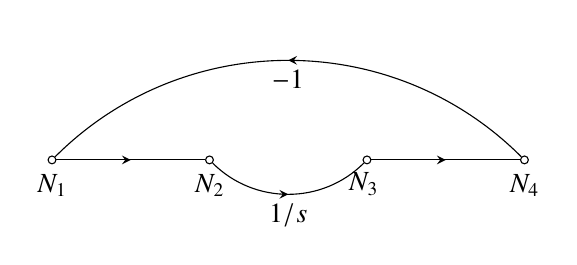
\begin{tikzpicture}
[
label revd/.is if=labrev,
amark/.style={
            decoration={             
                        markings,   
                        mark=at position {0.5} with { 
                                    \arrow{stealth},
                                    \iflabrev \node[above] {#1};\else \node[below] {#1};\fi
                        }
            },
            postaction={decorate}
},
terminal/.style 2 args={draw,circle,inner sep=1pt,label={#1:#2}},
]

%Place the nodes
%\node[terminal={below}{$X(s)$}] (a) at (0,0) {};
\node[terminal={below}{$N_1$}] (b) at (2cm,0) {};
\node[terminal={below}{$N_2$}] (c) at (4cm,0) {};
\node[terminal={[xshift=-4mm]below right}{$N_3$}] (d) at (6cm,0) {};
\node[terminal={below}{$N_4$}] (e) at (8cm,0) {};
%\node[terminal={below left}{$N_5$}] (f) at (11cm,0) {};
%\node[terminal={below left}{$Y(s)$}] (g) at (13cm,0) {};
%Draw the connections
%\draw[amark=$ $] (a) to (b);
\draw[amark=$ $] (b) to (c);
%\draw[amark=$s$] (c) to[bend left=45] (d);
%\draw[amark=$1/s$] (e) to (f);
%\draw[amark=$ $] (f) to (g);
\draw[amark=$ $] (d) to (e);
\draw[amark=$1/s$] (c) to[bend left=-45] (d);
\draw[amark=$-1$] (e) to[bend left=-45] (b);
%\draw[amark=$-1$,label revd] (f) to[bend left=50] (b);
%\draw[amark=$-K/M$,label revd] (e) to[bend right=50] (c);
\end{tikzpicture}
\caption{$L_3$}
\label{fig:sec_order}
\end{figure}


\begin{align}
L_4=(\frac{1}{s})(\frac{1}{s})(-1)=\frac{-1}{s^2}
\end{align}

\begin{figure}[!ht]
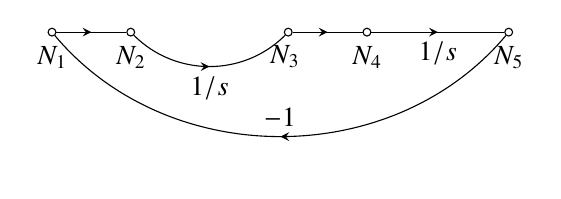
\begin{tikzpicture}
[
label revd/.is if=labrev,
amark/.style={
            decoration={             
                        markings,   
                        mark=at position {0.5} with { 
                                    \arrow{stealth},
                                    \iflabrev \node[above] {#1};\else \node[below] {#1};\fi
                        }
            },
            postaction={decorate}
},
terminal/.style 2 args={draw,circle,inner sep=1pt,label={#1:#2}},
]

%Place the nodes
%\node[terminal={below}{$X(s)$}] (a) at (0,0) {};
\node[terminal={below }{$N_1$}] (b) at (0,0) {};
\node[terminal={below }{$N_2$}] (c) at (1cm,0) {};
\node[terminal={[xshift=-4mm]below right}{$N_3$}] (d) at (3cm,0) {};
\node[terminal={below}{$N_4$}] (e) at (4cm,0) {};
\node[terminal={below}{$N_5$}] (f) at (5.8cm,0) {};
%\node[terminal={below left}{$Y(s)$}] (g) at (13cm,0) {};
%Draw the connections
%\draw[amark=$ $] (a) to (b);
\draw[amark=$ $] (b) to (c);
%\draw[amark=$s$] (c) to[bend left=45] (d);
\draw[amark=$1/s$] (e) to (f);
%\draw[amark=$ $] (f) to (g);
\draw[amark=$ $] (d) to (e);
\draw[amark=$1/s$] (c) to[bend left=-45] (d);
%\draw[amark=$-1$] (e) to[bend left=-45] (b);
\draw[amark=$-1$,label revd] (f) to[bend left=50] (b);
%\draw[amark=$-K/M$,label revd] (e) to[bend right=50] (c);
\end{tikzpicture}
\caption{$L_4$}
\label{fig:sec_order}
\end{figure}

\renewcommand{\thefigure}{\theenumi}

\item State Mason's Gain formula and explain the parameters through a table.
\\
\solution 
According to Mason's Gain Formula,
\begin{align}
T = \frac{Y(s)}{X(s)} 
\end{align}
\begin{align}
T = \frac{\sum_{i=1}^{N} P_i\Delta_i}{\Delta}
\end{align}
\item  Find the transfer function using Mason's Gain Formula.
\renewcommand{\thefigure}{\theenumi.\arabic{figure}}
%
\\
\solution 
%\begin{align}
% H(s)=\frac{Y(s)}{X(s)} 
%\end{align}

%Options -
% \begin{align}
% (A) - H(s)=\frac{s^2+1}{s^3+s^2+s+1}
% \end{align}
% \begin{align}
% (B) - H(s)=\frac{s^2+1}{s^3+2s^2+s+1}
% \end{align}
% \begin{align}
% (C) - H(s)=\frac{s^2+1}{s^2+s+1}
% \end{align}
% \begin{align}
% (D) - H(s)=\frac{s^2+1}{2s^2+1}
% \end{align}



Now, 

$P_i$ is the $i^{th}$ forward path.

$\Delta$ = 1 - (Sum of all individual loop gains)+(sum of gain products of all possible two non-touching loops)-(sum of gain products of all possible three non-touching loops)+...

$\Delta_i$ is  obtained from $\Delta$ by removing the loops which are touching the $i^{th}$ forward path.


$\Delta = 1-(L_1 + L_2 + L_3 + L_4)$

\begin{align}
L_1=(-1)(s)=-s
\end{align}

\begin{figure}[!ht]
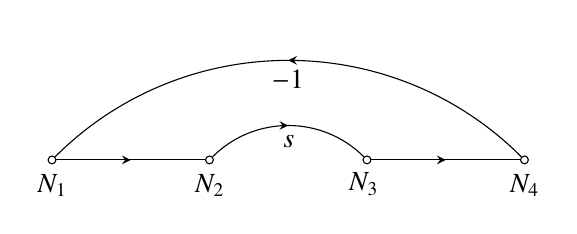
\begin{tikzpicture}
[
label revd/.is if=labrev,
amark/.style={
            decoration={             
                        markings,   
                        mark=at position {0.5} with { 
                                    \arrow{stealth},
                                    \iflabrev \node[above] {#1};\else \node[below] {#1};\fi
                        }
            },
            postaction={decorate}
},
terminal/.style 2 args={draw,circle,inner sep=1pt,label={#1:#2}},
]

%Place the nodes
%\node[terminal={below}{$X(s)$}] (a) at (0,0) {};
\node[terminal={below}{$N_1$}] (b) at (2cm,0) {};
\node[terminal={below}{$N_2$}] (c) at (4cm,0) {};
\node[terminal={[xshift=-4mm]below right}{$N_3$}] (d) at (6cm,0) {};
\node[terminal={below}{$N_4$}] (e) at (8cm,0) {};
%\node[terminal={below left}{$N_5$}] (f) at (11cm,0) {};
%\node[terminal={below left}{$Y(s)$}] (g) at (13cm,0) {};
%Draw the connections
%\draw[amark=$ $] (a) to (b);
\draw[amark=$ $] (b) to (c);
\draw[amark=$s$] (c) to[bend left=45] (d);
%\draw[amark=$1/s$] (e) to (f);
%\draw[amark=$ $] (f) to (g);
\draw[amark=$ $] (d) to (e);
%\draw[amark=$1/s$] (c) to[bend left=-45] (d);
\draw[amark=$-1$] (e) to[bend left=-45] (b);
%\draw[amark=$-1$,label revd] (f) to[bend left=50] (b);
%\draw[amark=$-K/M$,label revd] (e) to[bend right=50] (c);
\end{tikzpicture}
\caption{$L_1$}
\label{fig:sec_order}
\end{figure}


\begin{align}
L_2=\frac{s}{-s}=-1
\end{align}

\begin{figure}[!ht]
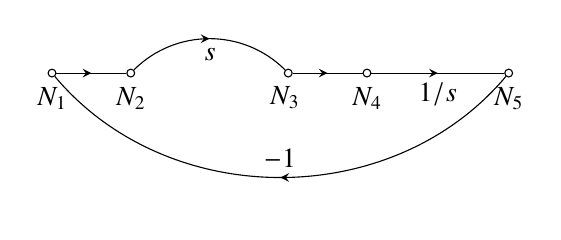
\begin{tikzpicture}
[
label revd/.is if=labrev,
amark/.style={
            decoration={             
                        markings,   
                        mark=at position {0.5} with { 
                                    \arrow{stealth},
                                    \iflabrev \node[above] {#1};\else \node[below] {#1};\fi
                        }
            },
            postaction={decorate}
},
terminal/.style 2 args={draw,circle,inner sep=1pt,label={#1:#2}},
]

%Place the nodes
%\node[terminal={below}{$X(s)$}] (a) at (0,0) {};
\node[terminal={below}{$N_1$}] (b) at (0,0) {};
\node[terminal={below}{$N_2$}] (c) at (1cm,0) {};
\node[terminal={[xshift=-4mm]below right}{$N_3$}] (d) at (3cm,0) {};
\node[terminal={below}{$N_4$}] (e) at (4cm,0) {};
\node[terminal={below}{$N_5$}] (f) at (5.8cm,0) {};
%\node[terminal={below left}{$Y(s)$}] (g) at (13cm,0) {};
%Draw the connections
%\draw[amark=$ $] (a) to (b);
\draw[amark=$ $] (b) to (c);
\draw[amark=$s$] (c) to[bend left=45] (d);
\draw[amark=$1/s$] (e) to (f);
%\draw[amark=$ $] (f) to (g);
\draw[amark=$ $] (d) to (e);
%\draw[amark=$1/s$] (c) to[bend left=-45] (d);
%\draw[amark=$-1$] (e) to[bend left=-45] (b);
\draw[amark=$-1$,label revd] (f) to[bend left=50] (b);
%\draw[amark=$-K/M$,label revd] (e) to[bend right=50] (c);
\end{tikzpicture}
\caption{$L_2$}
\label{fig:sec_order}
\end{figure}


\begin{align}
L_3=(\frac{1}{s})*(-1)=\frac{-1}{s}
\end{align}

\begin{figure}[!ht]
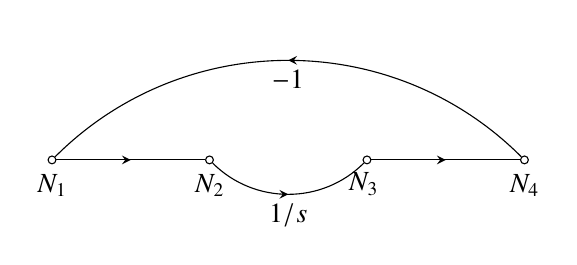
\begin{tikzpicture}
[
label revd/.is if=labrev,
amark/.style={
            decoration={             
                        markings,   
                        mark=at position {0.5} with { 
                                    \arrow{stealth},
                                    \iflabrev \node[above] {#1};\else \node[below] {#1};\fi
                        }
            },
            postaction={decorate}
},
terminal/.style 2 args={draw,circle,inner sep=1pt,label={#1:#2}},
]

%Place the nodes
%\node[terminal={below}{$X(s)$}] (a) at (0,0) {};
\node[terminal={below}{$N_1$}] (b) at (2cm,0) {};
\node[terminal={below}{$N_2$}] (c) at (4cm,0) {};
\node[terminal={[xshift=-4mm]below right}{$N_3$}] (d) at (6cm,0) {};
\node[terminal={below}{$N_4$}] (e) at (8cm,0) {};
%\node[terminal={below left}{$N_5$}] (f) at (11cm,0) {};
%\node[terminal={below left}{$Y(s)$}] (g) at (13cm,0) {};
%Draw the connections
%\draw[amark=$ $] (a) to (b);
\draw[amark=$ $] (b) to (c);
%\draw[amark=$s$] (c) to[bend left=45] (d);
%\draw[amark=$1/s$] (e) to (f);
%\draw[amark=$ $] (f) to (g);
\draw[amark=$ $] (d) to (e);
\draw[amark=$1/s$] (c) to[bend left=-45] (d);
\draw[amark=$-1$] (e) to[bend left=-45] (b);
%\draw[amark=$-1$,label revd] (f) to[bend left=50] (b);
%\draw[amark=$-K/M$,label revd] (e) to[bend right=50] (c);
\end{tikzpicture}
\caption{$L_3$}
\label{fig:sec_order}
\end{figure}


\begin{align}
L_4=(\frac{1}{s})(\frac{1}{s})(-1)=\frac{-1}{s^2}
\end{align}

\begin{figure}[!ht]
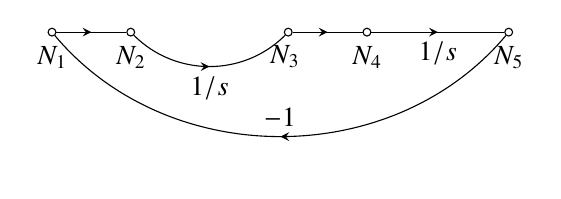
\begin{tikzpicture}
[
label revd/.is if=labrev,
amark/.style={
            decoration={             
                        markings,   
                        mark=at position {0.5} with { 
                                    \arrow{stealth},
                                    \iflabrev \node[above] {#1};\else \node[below] {#1};\fi
                        }
            },
            postaction={decorate}
},
terminal/.style 2 args={draw,circle,inner sep=1pt,label={#1:#2}},
]

%Place the nodes
%\node[terminal={below}{$X(s)$}] (a) at (0,0) {};
\node[terminal={below }{$N_1$}] (b) at (0,0) {};
\node[terminal={below }{$N_2$}] (c) at (1cm,0) {};
\node[terminal={[xshift=-4mm]below right}{$N_3$}] (d) at (3cm,0) {};
\node[terminal={below}{$N_4$}] (e) at (4cm,0) {};
\node[terminal={below}{$N_5$}] (f) at (5.8cm,0) {};
%\node[terminal={below left}{$Y(s)$}] (g) at (13cm,0) {};
%Draw the connections
%\draw[amark=$ $] (a) to (b);
\draw[amark=$ $] (b) to (c);
%\draw[amark=$s$] (c) to[bend left=45] (d);
\draw[amark=$1/s$] (e) to (f);
%\draw[amark=$ $] (f) to (g);
\draw[amark=$ $] (d) to (e);
\draw[amark=$1/s$] (c) to[bend left=-45] (d);
%\draw[amark=$-1$] (e) to[bend left=-45] (b);
\draw[amark=$-1$,label revd] (f) to[bend left=50] (b);
%\draw[amark=$-K/M$,label revd] (e) to[bend right=50] (c);
\end{tikzpicture}
\caption{$L_4$}
\label{fig:sec_order}
\end{figure}


$\Delta = 1-(-s-1-\frac{1}{s}-\frac{1}{s^2})$
$\Delta = \frac{s^3+2s^2+s+1}{s^2}$

\begin{figure}[!ht]
\begin{tikzpicture}
[
label revd/.is if=labrev,
amark/.style={
            decoration={             
                        markings,   
                        mark=at position {0.5} with { 
                                    \arrow{stealth},
                                    \iflabrev \node[above] {#1};\else \node[below] {#1};\fi
                        }
            },
            postaction={decorate}
},
terminal/.style 2 args={draw,circle,inner sep=1pt,label={#1:#2}},
]

%Place the nodes
%\node[terminal={below}{$X(s)$}] (a) at (0,0) {};
\node[terminal={below}{$N_1$}] (b) at (2cm,0) {};
%\node[terminal={below left}{$N_2$}] (c) at (4cm,0) {};
%\node[terminal={[xshift=-4mm]below right}{$N_3$}] (d) at (6cm,0) {};
\node[terminal={below}{$N_4$}] (e) at (8cm,0) {};
%\node[terminal={below left}{$N_5$}] (f) at (11cm,0) {};
%\node[terminal={below left}{$Y(s)$}] (g) at (13cm,0) {};
%Draw the connections
%\draw[amark=$ $] (a) to (b);
%\draw[amark=$ $] (b) to (c);
%\draw[amark=$s$] (c) to[bend left=45] (d);
%\draw[amark=$1/s$] (e) to (f);
%\draw[amark=$ $] (f) to (g);
%\draw[amark=$ $] (d) to (e);
%\draw[amark=$1/s$] (c) to[bend left=-45] (d);
\draw[amark=$-1$] (e) to[bend left=-45] (b);
%\draw[amark=$-1$,label revd] (f) to[bend left=50] (b);
%\draw[amark=$-K/M$,label revd] (e) to[bend right=50] (c);
\end{tikzpicture}
\caption{$\Delta_1$}
\label{fig:sec_order}
\end{figure}

After removing forward path from loop1 we will get Delta1

$\Delta_1 = 1$

\begin{figure}[!ht]
\begin{tikzpicture}
[
label revd/.is if=labrev,
amark/.style={
            decoration={             
                        markings,   
                        mark=at position {0.5} with { 
                                    \arrow{stealth},
                                    \iflabrev \node[above] {#1};\else \node[below] {#1};\fi
                        }
            },
            postaction={decorate}
},
terminal/.style 2 args={draw,circle,inner sep=1pt,label={#1:#2}},
]

%Place the nodes
%\node[terminal={below}{$X(s)$}] (a) at (0,0) {};
\node[terminal={below}{$N_1$}] (b) at (2cm,0) {};
%\node[terminal={below left}{$N_2$}] (c) at (4cm,0) {};
%\node[terminal={[xshift=-4mm]below right}{$N_3$}] (d) at (6cm,0) {};
%\node[terminal={below right}{$N_4$}] (e) at (8cm,0) {};
\node[terminal={below}{$N_5$}] (f) at (11cm,0) {};
%\node[terminal={below left}{$Y(s)$}] (g) at (13cm,0) {};
%Draw the connections
%\draw[amark=$ $] (a) to (b);
%\draw[amark=$ $] (b) to (c);
%\draw[amark=$s$] (c) to[bend left=45] (d);
%\draw[amark=$1/s$] (e) to (f);
%\draw[amark=$ $] (f) to (g);
%\draw[amark=$ $] (d) to (e);
%\draw[amark=$1/s$] (c) to[bend left=-45] (d);
%\draw[amark=$-1$] (e) to[bend left=-45] (b);
\draw[amark=$-1$,label revd] (f) to[bend left=50] (b);
%\draw[amark=$-K/M$,label revd] (e) to[bend right=50] (c);
\end{tikzpicture}
\caption{$\Delta_2$}
\label{fig:sec_order}
\end{figure}

After removing forward path from loop2 we will get Delta2

$\Delta_2 = 1$

\begin{figure}[!ht]
\begin{tikzpicture}
[
label revd/.is if=labrev,
amark/.style={
            decoration={             
                        markings,   
                        mark=at position {0.5} with { 
                                    \arrow{stealth},
                                    \iflabrev \node[above] {#1};\else \node[below] {#1};\fi
                        }
            },
            postaction={decorate}
},
terminal/.style 2 args={draw,circle,inner sep=1pt,label={#1:#2}},
]

%Place the nodes
%\node[terminal={below}{$X(s)$}] (a) at (0,0) {};
\node[terminal={below}{$N_1$}] (b) at (2cm,0) {};
%\node[terminal={below left}{$N_2$}] (c) at (4cm,0) {};
%\node[terminal={[xshift=-4mm]below right}{$N_3$}] (d) at (6cm,0) {};
\node[terminal={below}{$N_4$}] (e) at (8cm,0) {};
%\node[terminal={below left}{$N_5$}] (f) at (11cm,0) {};
%\node[terminal={below left}{$Y(s)$}] (g) at (13cm,0) {};
%Draw the connections
%\draw[amark=$ $] (a) to (b);
%\draw[amark=$ $] (b) to (c);
%\draw[amark=$s$] (c) to[bend left=45] (d);
%\draw[amark=$1/s$] (e) to (f);
%\draw[amark=$ $] (f) to (g);
%\draw[amark=$ $] (d) to (e);
%\draw[amark=$1/s$] (c) to[bend left=-45] (d);
\draw[amark=$-1$] (e) to[bend left=-45] (b);
%\draw[amark=$-1$,label revd] (f) to[bend left=50] (b);
%\draw[amark=$-K/M$,label revd] (e) to[bend right=50] (c);
\end{tikzpicture}
\caption{$\Delta_3$}
\label{fig:sec_order}
\end{figure}

After removing forward path from loop3 we will get Delta4

$\Delta_3 = 1$

\begin{figure}[!ht]
\begin{tikzpicture}
[
label revd/.is if=labrev,
amark/.style={
            decoration={             
                        markings,   
                        mark=at position {0.5} with { 
                                    \arrow{stealth},
                                    \iflabrev \node[above] {#1};\else \node[below] {#1};\fi
                        }
            },
            postaction={decorate}
},
terminal/.style 2 args={draw,circle,inner sep=1pt,label={#1:#2}},
]

%Place the nodes
%\node[terminal={below}{$X(s)$}] (a) at (0,0) {};
\node[terminal={below}{$N_1$}] (b) at (2cm,0) {};
%\node[terminal={below left}{$N_2$}] (c) at (4cm,0) {};
%\node[terminal={[xshift=-4mm]below right}{$N_3$}] (d) at (6cm,0) {};
%\node[terminal={below right}{$N_4$}] (e) at (8cm,0) {};
\node[terminal={below}{$N_5$}] (f) at (11cm,0) {};
%\node[terminal={below left}{$Y(s)$}] (g) at (13cm,0) {};
%Draw the connections
%\draw[amark=$ $] (a) to (b);
%\draw[amark=$ $] (b) to (c);
%\draw[amark=$s$] (c) to[bend left=45] (d);
%\draw[amark=$1/s$] (e) to (f);
%\draw[amark=$ $] (f) to (g);
%\draw[amark=$ $] (d) to (e);
%\draw[amark=$1/s$] (c) to[bend left=-45] (d);
%\draw[amark=$-1$] (e) to[bend left=-45] (b);
\draw[amark=$-1$,label revd] (f) to[bend left=50] (b);
%\draw[amark=$-K/M$,label revd] (e) to[bend right=50] (c);
\end{tikzpicture}
\caption{$\Delta_4$}
\label{fig:sec_order}
\end{figure}

After removing forward path from loop4 we will get Delta4

$\Delta_4 = 1$

Here, 
\begin{align}
T=\frac{\sum_{i=1}^{N}(P_i)(\Delta_i)}{\Delta}
\end{align}

\begin{align}
T=\frac{P_1 \Delta_1+P_2 \Delta_2+P_3 \Delta_3+P_4 \Delta_4}{\Delta}
\end{align}

\begin{align}
T=\frac{1*1 +(\frac{1}{s^2})*1 + 0*1 + 0*1 }{\frac{s^3+2s^2+s+1}{s^2}}
\end{align}

\begin{align}
H(s)=\frac{s^2+1}{s^3+2s^2+s+1}
\end{align}
\renewcommand{\thefigure}{\theenumi}

\end{enumerate}
\section{Routh Hurwitz Criterion}

\section{Compensators}
\section{Nyquist Plot}

%\section{Triangle}
%\subsection{Triangle Examples}
%\input{./triangle/tri_exam.tex} 
%\subsection{Triangle Exercises}
%\input{./triangle/tri_geo.tex} 
%%
%\section{Quadrilateral}
%\subsection{Quadrilateral Examples}
%\input{./quad/quad_geo_exam.tex} 
%\subsection{Quadrilateral Geometry}
%\input{./quad/quad_geo.tex} 
%
%\section{Constrained Optimization}
%%\subsection{Equality Constraint}
%\input{./chapters/line_exam.tex}
%\section{Convex Function}
%\input{./chapters/conv.tex}
%\section{Gradient Descent}
%\input{./chapters/grad_des.tex}
%\section{Lagrange Multipliers}
%\input{./chapters/lagrange.tex}
%\section{Quadratic Programming}
%\input{./chapters/qp.tex}
%\section{Semi Definite Programming}
%\input{./chapters/sdp.tex}
%\section{Linear Programming}
%\input{./chapters/lp_exam.tex}
%\section{Exercises}
%\input{./chapters/lp_exer.tex}


\end{document}


